
\documentclass[12pt, a4paper]{report}
\usepackage{graphicx}
\usepackage{amsmath}
\usepackage{float}
\usepackage{listings}


\title{\textbf{EE2703 : Applied Programming Lab \\ Assignment 3}} % Title

\author{Bachotti Sai Krishna Shanmukh \\ EE19B009} % Author name

\date{\today} % Date for the report

\begin{document}		
		
\maketitle % Insert the title, author and date
\section*{Questions 3 and 4}
 The plot of True values and noisy data is given in Figure 1  
 
 \begin{figure}[H]
	\centering
	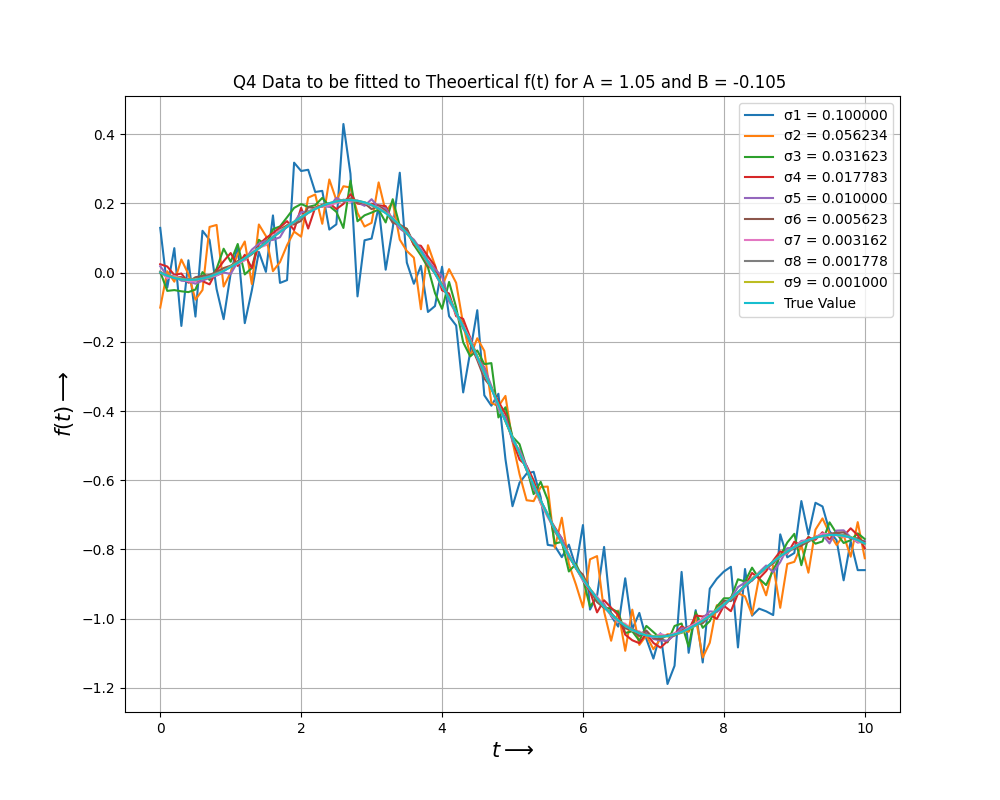
\includegraphics[scale=0.6]{Figure_0.png}  % Mention the image name within the curly braces. Image should be in the same folder as the tex file. 
	\caption{Plot for Q4}
	\label{fig:sample}
\end{figure} 

\section*{Question 5}
The plot in Figure 2 shows the error between True Values and the data corresponding to a noise of standard deviation $\sigma$ = 0.1

 \begin{figure}[H]
	\centering
	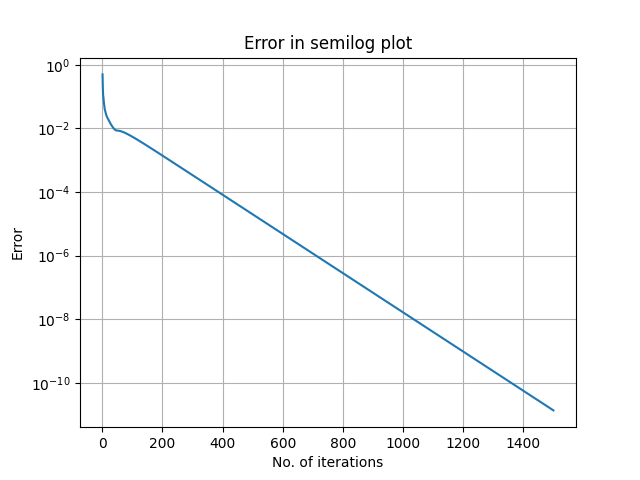
\includegraphics[scale=0.6]{Figure_1.png}  % Mention the image name within the curly braces. Image should be in the same folder as the tex file. 
	\caption{Plot for Q5}
	\label{fig:sample}
\end{figure} 

\section*{Question 6}
Using the function $array\_equal$ can return False value to arrays which are closely equal, but strictly unequal. This function may not be desirable in this case.
We can use the function $allclose$ in the NumPy module to check if the two arrays are element-wise equal within a tolerance
\lstinputlisting[language = Python, firstline = 76, lastline= 84]{EE2703_Assignment3_EE19B009.py}

The return value of this function will be True if nearly equal.

\section*{Question 8}
The contour plot of the mean squared error versus the parameters A and B is given in Figure 3. We can observe that a single minima is present in the plot

\begin{figure}[H]
	\centering
	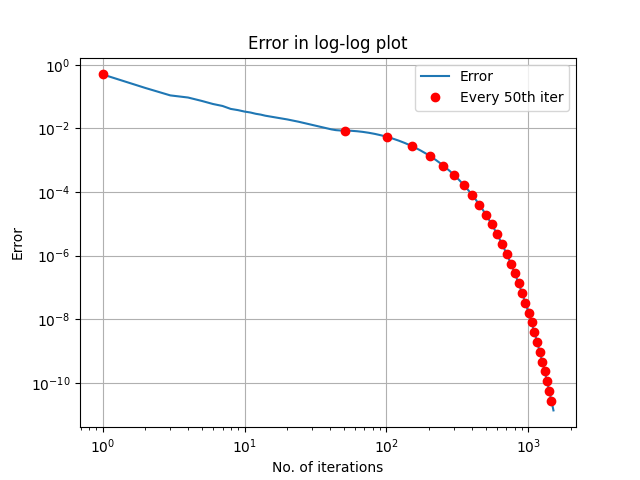
\includegraphics[scale=0.6]{Figure_2.png}  % Mention the image name within the curly braces. Image should be in the same folder as the tex file. 
	\caption{Plot for Q10}
	\label{fig:sample}
\end{figure} 

\section*{Question 10}

The plot of the error in the estimation of A and B parameters with respect to standard deviation ($\sigma$) of the noise is given in Figure 4

\begin{figure}[H]
	\centering
	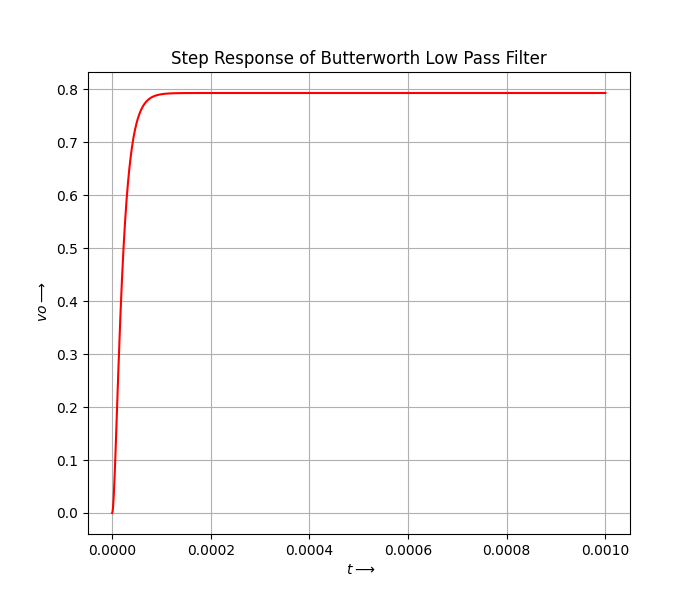
\includegraphics[scale=0.6]{Figure_3.png}  % Mention the image name within the curly braces. Image should be in the same folder as the tex file. 
	\caption{Plot for Q10}
	\label{fig:sample}
\end{figure} 

The error in estimate of A and B is growing with the noise in a non linear way.

\section*{Question 11}
The log-scale plot of error in estimation of A and B parameters with respect to standard deviation ($\sigma$) of the noise is given in Figure 5

\begin{figure}[H]
	\centering
	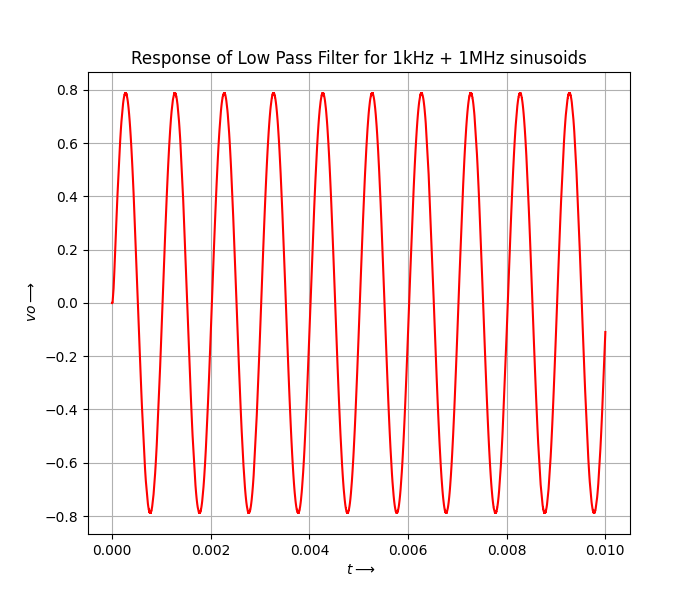
\includegraphics[scale=0.6]{Figure_4.png}  % Mention the image name within the curly braces. Image should be in the same folder as the tex file. 
	\caption{Plot for Q10}
	\label{fig:sample}
\end{figure} 

The error in estimation of A and B $vs$ standard deviation ($\sigma$) of noise has a better linear fit in log scale i.e., Figure 5 compared to the plot in Figure 4


\end{document}



 